% Szglab4
% ===========================================================================
%

\chapter{Követelmény, projekt, funkcionalitás}

\thispagestyle{fancy}

\section{Bevezetés}

\subsection{Cél}

\comment{A dokumentum célja.}

\subsection{Szakterület}

\comment{A kialakítandó szoftver milyen területen használható, milyen célra.}

\subsection{Definíciók, rövidítések}
\comment{A dokumentumban használt definíciók, rövidítések magyarázata.}

\subsection{Hivatkozások}
\comment{A dokumentumban használt anyagok, web-oldalak felsorolása}

\subsection{Összefoglalás}
\comment{A dokumentum további részeinek rövid ismertetése}

\section{Áttekintés}
\subsection{Általános áttekintés}
\comment{A kialakítandó szoftver legmagasabb szintű architekturális képe. A fontosabb alrendszerek felsorolása, a közöttük kialakítandó interfészek lényege, a felhasználói kapcsolatok alapja. Esetleges hálózati és adattárolási elvárások.}

\subsection{Funkciók}
\comment{A feladat kb. 4000 karakteres (kb 1,5 oldal) részletezettségű magyar nyelvű leírása. Nem szerepelhetnek informatikai kifejezések.}

\subsection{Felhasználók}
\comment{A felhasználók jellemzői, tulajdonságai}

\subsection{Korlátozások}
\comment{Az elkészítendő szoftverre vonatkozó – általában nem funkcionális - előírások, korlátozások.}

\subsection{Feltételezések, kapcsolatok}
\comment{A dokumentumban használt anyagok, web-oldalak felsorolása}

\section{Követelmények}
\subsection{Funkcionális követelmények}


\comment{Az alábbi táblázat kitöltésével készítendő. Dolgozzon ki követelmény azonosító rendszert! Az ellenőrzés módja szokásosan bemutatás és/vagy kiértékelés. Prioritás lehet alapvető, fontos, opcionális. Az alapvető követelmények nem teljesítése végzetes. Forrás alatt a követelményt előíró anyagot, szervezetet kell érteni. Esetünkben forrás lehet maga a csapat is, mikor ő talál ki követelményt. Use-case-ek alatt az adott követelményt megvalósító használati esete(ke)t kell megadni.}

% Azonosító, Leírás, Ellenőrzés, Prioritás, Forrás, Use-case, Komment
\begin{longtable}{| l | l | l | l | l | l | l |}
\hline
\textbf{Azonosító}   & \textbf{Leírás} & \textbf{Ellenőrzés} & \textbf{Prioritás} & \textbf{Forrás} & \textbf{Use-case} & \textbf{Komment} \tabularnewline
\hline\hline
... & ... & ... & ... & ... & ... & ... \tabularnewline
\hline
\end{longtable}

\subsection{Erőforrásokkal kapcsolatos követelmények}

\comment{A szoftver fejlesztésével és használatával kapcsolatos számítógépes, hardveres, alapszoftveres és egyéb architekturális és logisztikai követelmények}

% Azonosító, Leírás, Ellenőrzés, Prioritás, Forrás, Komment
\begin{longtable}{| l | l | l | l | l | l |}
\hline
\textbf{Azonosító}   & \textbf{Leírás} & \textbf{Ellenőrzés} & \textbf{Prioritás} & \textbf{Forrás} & \textbf{Komment} \tabularnewline
\hline\hline
... & ... & ... & ... & ... & ... \tabularnewline
\hline
\end{longtable}


\subsection{Átadással kapcsolatos követelmények}
\comment{A szoftver átadásával, telepítésével, üzembe helyezésével kapcsolatos követelmények}

% Azonosító, Leírás, Ellenőrzés, Prioritás, Forrás, Komment
\begin{longtable}{| l | l | l | l | l | l |}
\hline
\textbf{Azonosító}   & \textbf{Leírás} & \textbf{Ellenőrzés} & \textbf{Prioritás} & \textbf{Forrás} & \textbf{Komment} \tabularnewline
\hline\hline
... & ... & ... & ... & ... & ... \tabularnewline
\hline
\end{longtable}

\subsection{Egyéb nem funkcionális követelmények}
\comment{A biztonsággal, hordozhatósággal, megbízhatósággal, tesztelhetőséggel, a felhasználóval kapcsolatos követelmények}

% Azonosító, Leírás, Ellenőrzés, Prioritás, Forrás, Komment
\begin{longtable}{| l | l | l | l | l | l |}
\hline
\textbf{Azonosító}   & \textbf{Leírás} & \textbf{Ellenőrzés} & \textbf{Prioritás} & \textbf{Forrás} & \textbf{Komment} \tabularnewline
\hline\hline
... & ... & ... & ... & ... & ... \tabularnewline
\hline
\end{longtable}


\section{Lényeges use-case-ek}
\comment{A 2.3.1-ben felsorolt követelmények közül az alapvető és fontos követelményekhez tartozó használati esetek megadása az alábbi táblázatos formában.}

\subsection{Use-case leírások}

\usecase
{Új játék indítása}
{Új játék indul el}
{Játékos}
{1. A játékos kiválasztja a menüben az "Új játék" feliratú gombot, és megnyomja. \newline
2. Ezután kiválaszthatja  a nehézséget és a pályát. \newline
3. Elindul a játék a kiválasztott pályával és nehézséggel.}

\usecase
{Pálya kiválasztása}
{Ki kell választani a pályát amelyen játszani kíván.}
{Játékos}
{Új játék indítása után egy listából ki kell választani a pályát amelyen játszani kíván.}

\usecase
{Nehézségi szint kiválasztása}
{Ki kell választani, hogy milyen nehézségen kíván játszani.}
{Játékos}
{Új játék indítása, és a pálya kiválasztása után, ki kell választani három opció közül,
 hogy mennyire legyen a játék nehéz.}

\usecase
{Torony építése}
{Új tornyot épít}
{Játékos}
{Olyan mezőre kattintva, ahol nincsen út vagy torony, ott új torony épül, 
ha van elég varázserő hozzá.}

\usecase
{Akadály építése}
{Új akadályt épít}
{Játékos}
{Olyan mezőre kattintva ahol út van, és még nincsen akadály, ott akadály épül,
ha van elég varázserő hozzá.}

\usecase
{Torony/akadály enchant-olás}
{Már létező tornyot vagy akadályt enchant-olunk}
{Játékos}
{Toronyra vagy akadályra kattintva ki kell választani, hogy milyen drágakővel szeretné enchant-olni, 
és ha van elég varázserő hozzá akkor megtörténik az enchant.}

\usecase
{Feladás}
{Feladjuk a jelenlegi játékot}
{Játékos}
{A feladás gombra kattintva a játék végetér, és megnyílik a főmenü.}

\usecase
{Kilépés}
{Kilép az alkalmazásból}
{Játékos}
{Az ablak jobb felső sarkában, a bezárásra kattintva az alkalmazás kilép.}

\subsection{Use-case diagram}

\begin{figure}[ht!]
\centering
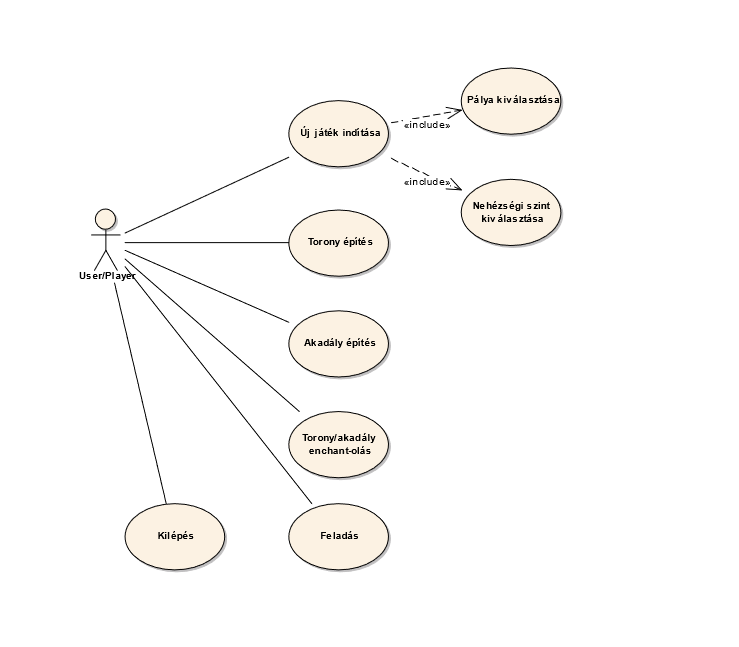
\includegraphics[width=170mm]{images/UseCase.png}
\caption{Use-case diagram}
\label{overflow}
\end{figure}

\section{Szótár}
\comment{A szótár a követelmények alapján készítendő fejezet. Egy szótári bejegyzés definiálásához csak más szótári bejegyzések és köznapi – a feladattól független – fogalmak használhatók fel. A szótár mérete kb. 1-2 oldal legyen.}

\section{Projekt terv}
\comment{Tartalmaznia kell a projekt végrehajtásának lépéseit, a lépések, eredmények határidejét, az egyes feladatok elvégzéséért felelős személyek nevét és beosztását, a szükséges erőforrásokat, stb. Meg kell adni a csoportmunkát támogató eszközöket, a választott technikákat! Definiálni kell, hogy hogyan történik a dokumentumok és a forráskód megosztása!}


